%
% einleitung.tex -- Beispiel-File für die Einleitung
%
% (c) 2020 Prof Dr Andreas Müller, Hochschule Rapperswil
%
\section{Lösungsmethode 3: Simulation 
	\label{kreismembran:section:teil4}}
\kopfrechts{Lösungsmethode 3: Simulation}
\index{Simulation}%
Um numerisch das Verhalten einer Membran zu ermitteln, muss eine
numerische Darstellung definiert werden.
Die Membran wird hier in Form der Matrix $  U $ digitalisiert.
Jedes Element  $ U_{ij} $ steht für die Auslenkung der Membran $
u(x,y,t) $ an der Stelle $(x,y)=(i,j) $.
Zwischen benachbarten Elementen in der Matrix $ U $ liegt immer der
Abstand $ dh $, eine Inkrementierung von $ i $ oder $ j $ ist somit
ein Schritt in Richtung $ x $ oder $ y $ von Länge $ dh $ auf der
Membran.
Die zeitliche Dimension wird in Form des Array $  U[] $ aus $ z
\times U $ Matrizen dargestellt, wobei $ z $ die Anzahl von
Zeitschritten ist.
Das Element auf Zeile $ i $, Spalte $ j $ der $ w $-ten Matrix von $ U[] $ also $ U[w]_{ij} $ ist somit die Auslenkung $ u(i,j,w) $.
Da die Differentialgleichung von zweiter Ordnung ist, reicht eine Zustandsvariabel pro Membran-Element nicht aus. 
Es wird neben der Auslenkung auch die Geschwindigkeit jedes Membran-Elementes benötigt um den Zustand eindeutig zu beschreiben. 
Dazu existiert neben $ U[] $ ein analoger Array $ V[] $, welcher die
Geschwindigkeiten aller Membran-Elemente repräsentiert.
$ V[w]_{ij} $ entspricht also $ \dot{u}(i,j,w) $. 
Der Zustand einer Membran zum Zeitpunkt $ w $ wird mit $ X[w] $ beschrieben, was $ U[w] $ und $ V[w] $ beinhaltet.

\subsection{Propagation}
\index{Propagation}%
Um das Verhalten der Membran zu berechnen, muss aus einem gegebenen Zustand $ X[w] $ der Folgezustand $ X[w+1] $ gerechnet werden können, wobei dazwischen ein Zeitintervall $ dt $ vergeht. 
Die Berechnung von Folgezuständen kann anschliessend wiederholt werden über
das zu untersuchende Zeitfenster.
Die Folgeposition $ U[w+1] $ ergibt sich als 
\begin{equation}
	U[w+1] =  U[w] + dt \cdot V[w],
\end{equation} 
also die Ausgangslage plus die Strecke welche während des Zeitintervall
mit der Geschwindigkeit des Elementes zurückgelegt wurde.
Dieses Verfahren wird Euler-Methode genannt.
\index{Euler-Methode}%

Neben der Position muss auch die Geschwindigkeit aktualisiert werden.
Analog zur Folgeposition wird
\begin{equation*}
	V[w+1] = V[w] + dt \cdot \frac{\partial^2u}{\partial t^2}.
\end{equation*}    
Die Beschleunigung $ \frac{\partial^2u}{\partial t^2} $  eines Elementes ist durch die Differentialgleichung \ref{kreismembran:Ausgang_DGL} gegeben als
\begin{equation*}
	\frac{\partial^2u}{\partial t^2} = \Delta u \cdot c^2.
\end{equation*}
Die Geschwindigkeit des Folgezustandes kann somit mit
\begin{equation}
	V[w+1] = V[w] + dt \cdot \Delta_h U \cdot c^2
\end{equation}
berechnet werden.
Während $ c^2 $ lediglich eine materialspezifische Konstante ist,
muss noch erläutert werden, wie der diskrete Laplace-Operator für
$ \Delta_h u $ definiert ist.

\subsection{Diskreter Laplace-Operator $\Delta_h$}
\index{Laplace-Operator, diskreter}%
Die diskrete Ableitung zweiter Ordnung kann mit Hilfe der Taylor-Reihen-Entwicklung als
\begin{equation*}
	\frac{\partial^2f}{\partial x^2} \approx \frac{f(x+dx)-2f(x)+f(x-dx)}{dx^2}
\end{equation*}
approximiert werden \cite{kreismembran:Digital_Image_processing}.
Dank der Linearität der Ableitung kann die Ableitung einer weiteren
Dimension hinzugefügt werden.
Daraus folgt für den zweidimensionalen Fall 
\begin{equation*}
	\Delta_h u= \frac{u(x+dh,y,t)+u(x,y+dh,t)-4f(x)+u(x-dh,y,t)+u(x,y-dh,t)}{dh^2}.
\end{equation*}
Um $ \Delta_h $ auf eine Matrix anwenden zu können wird die Gleichung
in Form einer Filtermaske 
\index{Filtermaske}%
\begin{equation}
 	\Delta_h u= \frac{1}{dh^2}
 	\left[ {\begin{array}{ccc}
 			0 & 1  & 0\\
 			1 & -4 & 1\\
 			0 & 1  & 0\\
 	\end{array} } \right]
\end{equation}
formuliert.
Die Filtermaske kann dann mit einer Matrizen-Faltung
auf jedes Element einzeln angewendet werden,
um $ \Delta_h U[] $ zu berechnen.

\subsection{Simulation: Kreisförmige Membran}
Als Beispiel soll nun eine schwingende kreisförmige Membran simuliert werden.
\subsubsection{Initialisierung}
Die Anzahl der simulierten Elemente soll $ m \times n $ sein, was die Dimensionen von $ U $ und $ V $ vorgibt.
Als Anfangsbedingung wird eine Membran gewählt, welche bei $ t=0 $ mit einer Gauss-Kurve ausgelenkt wird.
Die Membran soll sich zu Beginn nicht bewegen, also wird $ V[0] $ mit Nullen initialisiert.
Die Auslenkung kann kompakt erreicht werden, wenn $ U[0] $ als Null-Matrix mit einer $ 1 $ in der Mitte initialisiert wird. 
Diese Matrix wird anschliessend mit einer Filtermaske in Form einer Gauss-Glocke gefaltet.
Die Faltung mit einer Gauss-Glocke ist in Programmen wie Matlab eine Standartfunktion, da dies einem Tiefpassfilter in der Bildverarbeitung entspricht.

\subsubsection{Rand}
Bislang ist die definierte Matrix rechteckig.
Um eine kreisförmige Membran zu simulieren, muss der Rand angepasst werden.
Da in den meisten Programme keine Möglichkeit besteht, mit runden Matrizen zu rechnen, wird der Rand in der Berechnung des Folgezustandes implementiert.
Der Rand bedeutet, dass Membran-Elemente auf dem Rand sich nicht
bewegen können.
Die Position sowie die Geschwindigkeit aller Elemente, welche nicht
auf der definierten Membran sind, müssen zu beliebiger Zeit $0$ sein.
Hierzu wird eine Maske $M$ erstellt. 
Diese Maske besteht aus einer binären Matrix von identischer Dimension
wie $ U $ und $ V $. 
Ist in der Matrix $M$ eine $1$ abgebildet, so ist an jener Stelle ein Element der Membran, ist es eine $0$ so befindet sich dieses Element auf dem Rand oder ausserhalb der Membran.
In dieser Anwendung ist $M$ eine Matrix mit einem Kreis voller $1$ umgeben von $0$ bis an den Rand der Matrix.
Die Maske wird angewendet, indem das Resultat des nächsten Zustandes noch mit der Maske elementweise multipliziert wird. 
Der Folgezustand kann also mit den Gleichungen
\begin{align}
	\label{kreismembran:eq:folge_U} 
	U[w+1] &= (U[w] + dt \cdot V[w])\odot M\\
	\label{kreismembran:eq:folge_V}
	V[w+1] &= (V[w] + dt \cdot \Delta_h u \cdot c^2)\odot M
\end{align}
berechnet werden.
Das Symbol $\odot$ steht hier für eine elementweise Matrixmultiplikation
(Hadamard-Produkt)
\index{Hadamard-Produkt}%

\subsubsection{Simulation}
Mit den gegebenen Gleichungen \eqref{kreismembran:eq:folge_U} und
\eqref{kreismembran:eq:folge_V} kann das Verhalten der Membran mit einem
Loop über das zu untersuchende Zeitintervall berechnet werden. 
In der Abbildung \ref{kreismembran:im:simres_rund} sind Simulationsresultate zu sehen.
Die erste Figur zeigt die Ausgangslage gefolgt von den Auslenkungen nach jeweils $ 50 $ weiteren Iterationsschritten.
Es ist zu erkennen, wie sich die Störung vom Zentrum an den Rand ausbreitet.
Erreicht die Störung den Rand, wird sie reflektiert und nähert sich dem Zentrum. 
\begin{figure}
	
	\begin{center}
		
		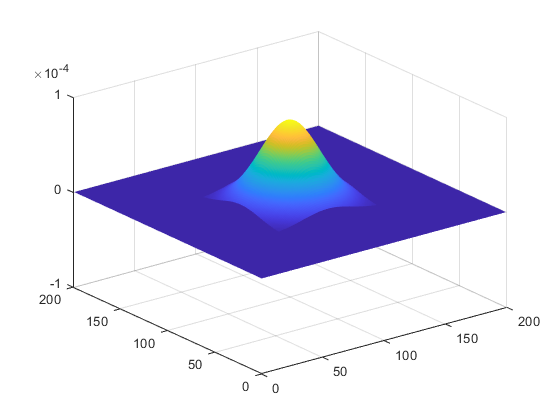
\includegraphics[width=0.32\textwidth]{papers/kreismembran/images/sim_1_1.png}
		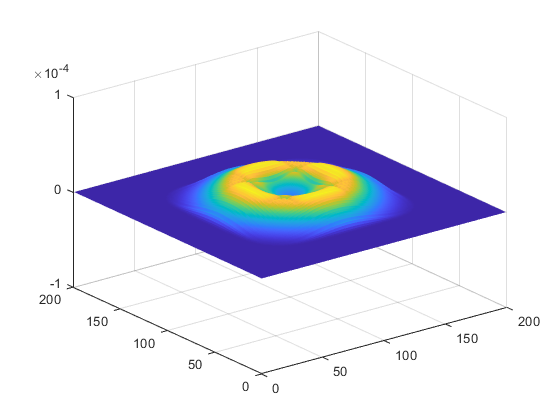
\includegraphics[width=0.32\textwidth]{papers/kreismembran/images/sim_1_2.png}
		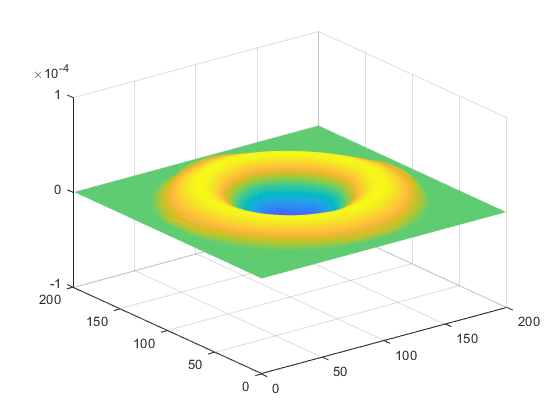
\includegraphics[width=0.32\textwidth]{papers/kreismembran/images/sim_1_3.png}
		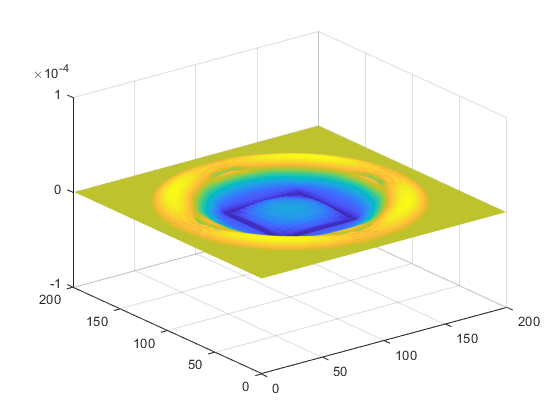
\includegraphics[width=0.32\textwidth]{papers/kreismembran/images/sim_1_4.png}
		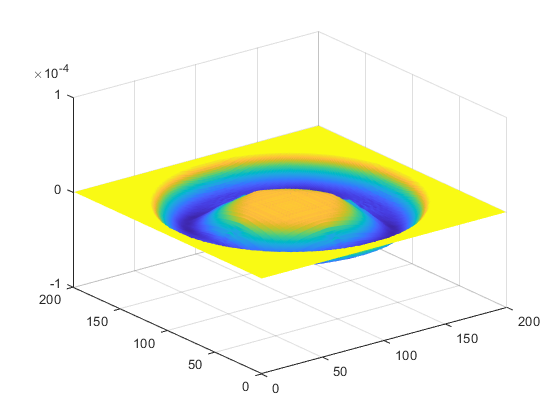
\includegraphics[width=0.32\textwidth]{papers/kreismembran/images/sim_1_5.png}
		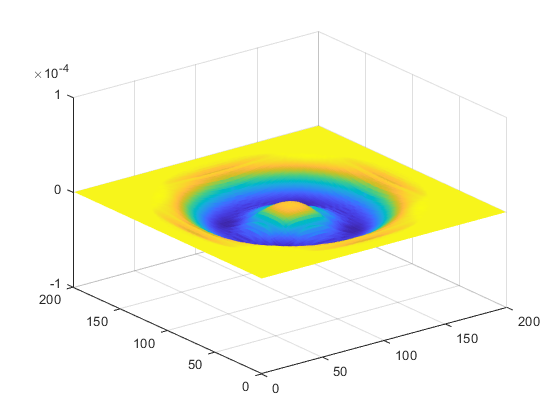
\includegraphics[width=0.32\textwidth]{papers/kreismembran/images/sim_1_6.png}
		\caption{Simulations Resultate einer kreisförmigen Membran. Simuliert mit $ 200 \times 200 $ Elementen, dargestellt sind die Auslenkungen nach jeweils $ 50 $ Iterationsschritten.}
		\label{kreismembran:im:simres_rund}
		
	\end{center}	
\end{figure} 
\subsection{Simulation: Unendliche Membran}
Um eine unendlich grosse Membran zu simulieren, könnte der unpraktische Weg gewählt werden, die Matrix unendlich gross zu definieren, dies wird jedoch spätestens bei der numerischen Berechnung seine Probleme mit sich bringen.
Etwas geeigneter ist es, die Matrix so gross wie möglich zu definieren, wie es die Kapazitäten erlauben.
Wenn anschliessend nur das Verhalten im Zentrum, bei der Störung beobachtet wird, verhaltet sich die Membran wie eine unendliche. 
Dies aber nur bis die Störung am Rand reflektiert wird und wieder das Zentrum beeinflusst.
Soll erst gar keine Reflexion entstehen, muss ein Absorber modelliert werden welcher die Störung möglichst ohne Reflexion aufnimmt.

\subsubsection{Absorber}
\index{Absorber}%
Sehr knapp formuliert entstehen Reflexionen, wenn eine Welle von einem Material in ein anderes Material mit unterschiedlichen Eigenschaften eindringen möchte.
Je unterschiedlicher und abrupter der Übergang zwischen den Materialien umso ausgeprägter die Reflexion.
In diesem Fall sind die Eigenschaften vorgegeben.
Im Zentrum soll sich die Membran verhalten, wie von der Differentialgleichung vorgegeben, am Rand jedoch muss sich jedes Membran-Element in der Ausgangslage befinden. 
Der Spielraum, welcher dem Absorber übrig bleibt, ist die Art der Überganges.
Bei der endlichen kreisförmigen Membran hat die Maske $M$ einen binären Übergang von Membran zu Rand bezweckt.
Anstelle dieses abrupten Wechsels wird nun eine Maske definiert, welche graduell von Membran $1$ zu Rand-Element $0$ wechselt.
Die Elemente werden auf Basis ihres Abstand $r$ zum Zentrum definiert. 
Der Abstand ist 
\begin{equation*}
	r(i,j)
	=
	\sqrt{\biggl|i-\frac{m}{2}\biggr|^2+\biggl|j-\frac{n}{2}\biggr|^2},
\end{equation*} 
wobei $ m $ und $n$ die Dimensionen der Matrix sind.
Für einen stufenlosen Übergang werden die Elemente der Maske auf 

\begin{align}
	M_{ij} = \begin{cases} 1-e^{(r(i,j)-b)a} & \text{$x > b$} \\
		0 & \text{sonst} \end{cases}
\end{align}
gesetzt.
Der Parameter $a > 0$ bestimmt wie steil der Übergang sein soll, $b$ bestimmt  wie weit weg vom Zentrum sich der Übergang befindet.
In der Abbildung \ref{kreismembran:im:masks} ist der Unterschied der beiden Masken zu sehen. 
\begin{figure}
	
	\begin{center}
		
		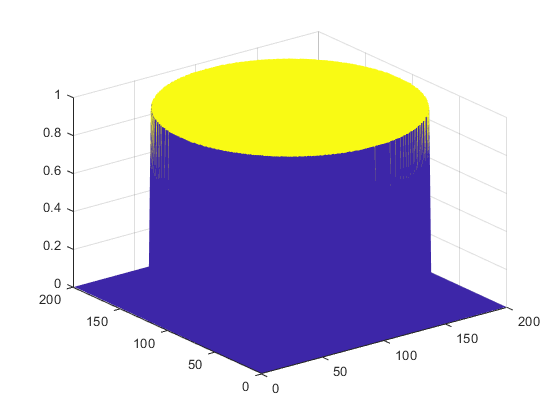
\includegraphics[width=0.45\textwidth]{papers/kreismembran/images/mask_disk.png}
		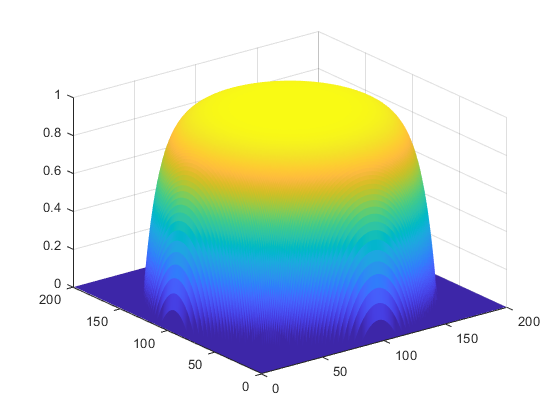
\includegraphics[width=0.45\textwidth]{papers/kreismembran/images/mask_absorber.png}
		\caption{Vergleich von Masken: Links Binär für eine endliche Membran, rechts mit Absorber für eine unendliche Membran}
		\label{kreismembran:im:masks}
	\end{center}	
\end{figure} 
\subsubsection{Simulation}
Bis auf die Absorber-Maske kann nun identisch zur endlichen Membran
simuliert werden.
Auch hier wurde eine Gauss-Glocke als Anfangsbedingung gewählt. 
Die Simulationsresultate von Abbildung \ref{kreismembran:im:simres_unendlich}
\begin{figure}
	
	\begin{center}
		
		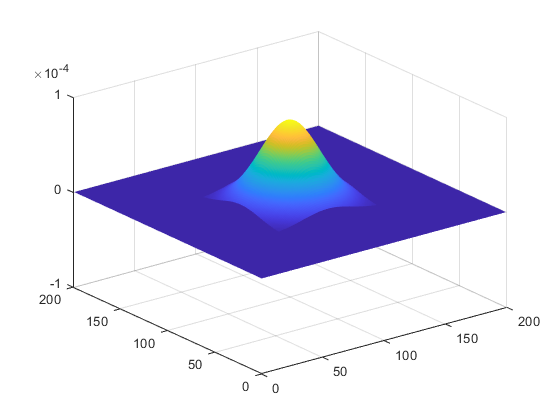
\includegraphics[width=0.32\textwidth]{papers/kreismembran/images/sim_2_1.png}
		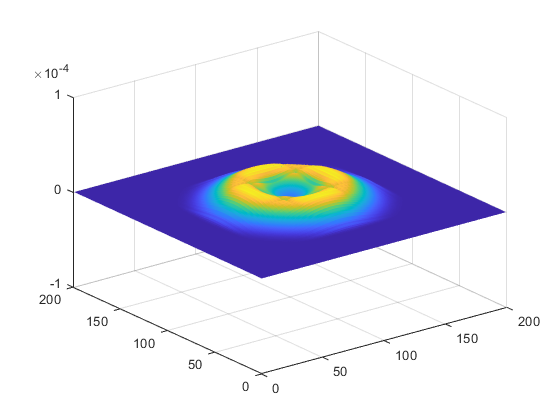
\includegraphics[width=0.32\textwidth]{papers/kreismembran/images/sim_2_2.png}
		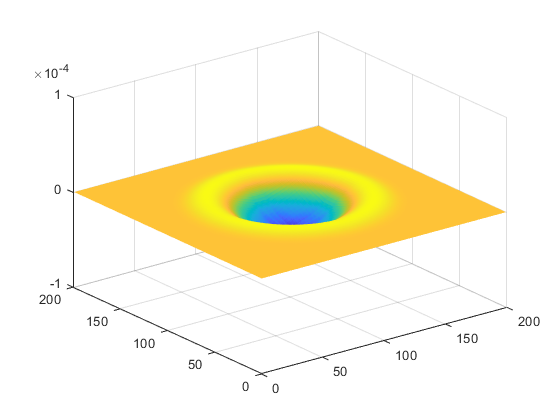
\includegraphics[width=0.32\textwidth]{papers/kreismembran/images/sim_2_3.png}
		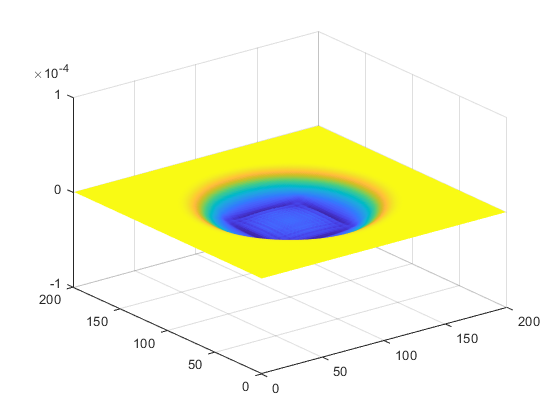
\includegraphics[width=0.32\textwidth]{papers/kreismembran/images/sim_2_4.png}
		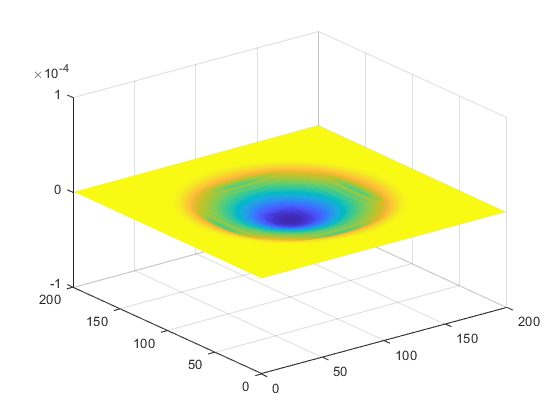
\includegraphics[width=0.32\textwidth]{papers/kreismembran/images/sim_2_5.png}
		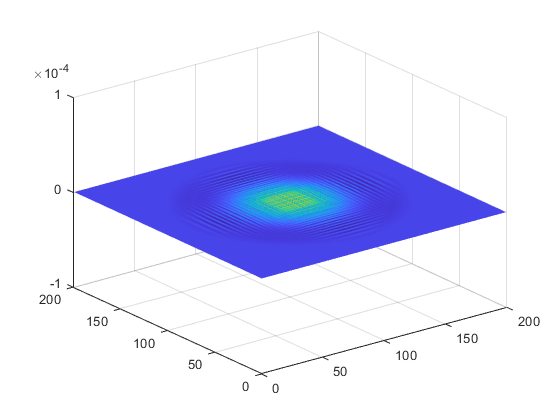
\includegraphics[width=0.32\textwidth]{papers/kreismembran/images/sim_2_6.png}
		\caption{Simulations Resultate einer unendlichen Membran. Simuliert mit $ 200 \times 200 $ Elementen, dargestellt sind die Auslenkungen nach jeweils $ 50 $ Iterationsschritten.}
		\label{kreismembran:im:simres_unendlich}
		
	\end{center}	
\end{figure}
zeigen deutlich, wie die Störung vom Zentrum weg verläuft.
Nähert sich die Störung dem Rand, so wird sie immer stärker abgeschwächt.
Die Wirkung des Absorber ist an der letzten Figur zu erkennen, in welcher kaum noch Auslenkungen zu sehen sind.
Dieses Verhalten spricht für den Absorber-Ansatz, es soll jedoch erwähnt sein, dass der Übergangsbereich eine sanft ansteigende Dämpfung in das System bringt.
Die Differentialgleichung \eqref{kreismembran:Ausgang_DGL}, welche
simuliert wird, geht jedoch von der Annahme \ref{kreimembran:annahmen}
iv) aus, dass die Membran keine Art von Dämpfung erfährt.

\section{Schlusswort}
\kopfrechts{Schlusswort}
Auch wenn ein physikalisches Verhalten bereits durch Annahmen und
Annäherungen deutlich vereinfacht wird, bestehen auch dann noch
eine Vielzahl von Lösungsansätzen.
Lösungen einer unendlich grosse Membran scheinen fern der Realität
zu sein, doch dies darf es im Sinne der Mathematik.
Und wer weiss, für eine Ameise auf einem Trampolin ist eine unendliche
\index{Ameise}%
\index{Trampolin}%
Membran vielleicht eine ganz gute Annäherung.






